\chapter{Non-Resonance 7 TeV Analysis}

This chapter looks at the non-resonant analysis done within ATLAS on 2011 data and precursor to the main analysis in this thesis. It is noticeable that this thesis lacks many parts of the 2012 analysis such as angular search in $\cos{\theta^{*}}$ and searches for only the LL CI formalism and GRW ADD formalism. The analysis was published in the paper found here \cite{PhysRevD.87.015010}. 


%comparisons between analyses


\section{Data and Background Processes}

\subsection{Data}
	All data used in the CI analysis is taken from the LHC 2011 $\sqrt{s} = 7 TeV$ proton-proton collision data  of which ATLAS recorded $4.9 fb^{-1}$ of electron candidate data. Data was collected with stable LHC beams and a fully operational inner detector and calorimeter each being important in the identification of good electron candidates.

\subsection{Background}
	The main background the CI signal in the electron channel is Drell-Yan (DY) $\rightarrow~ee$ production mediated by a photon or the Z boson. However there are other small contributions from $t\bar{t}$, diboson, W + jets and QCD production. $t\bar{t}$ background consists of events with $t\bar{t}$ production decaying to amongst other things two electrons. Diboson background can involve either an event producing two W bosons, two Z boson or one W and one Z boson in which two electrons also exist in the final decay state. Both these productions can result in two electrons with a large combined invariant mass which could mimic CI production. W + jets production can result in an electron and a jet faking an electron left in the final state, while QCD refers to events where two jets fake electrons. These all combine to form the background sample.

\subsection{Background Production}
	Contributions from SM processes were primarily simulated via leading-order (LO) $PYTHIA$ \cite{pythia} Monte Carlo (MC) event generation and using $Geant 4$ \cite{geant} to simulate the ATLAS detector. This method was used to generate a $Z\rightarrow~ee$ sample for the low dielectron invariant mass region ($m_{ee} < 120 GeV$) and a $DY\rightarrow~ee$ mass binned sample for the invariant high mass ($m_{ee} > 120 GeV$) to keep high statistics at high invariant mass. Four other samples are included to produce the background estimate, these are $t\bar{t}$ (produced with $MC@NLO$), diboson(WW, WZ and ZZ decays produced with $HERWIG$), W + jets (produced with $ALPGEN$, $JIMMY$ and $HERWIG$) and QCD (produced using a data driven method \cite{QCD}).

\subsection{Signal} 

	Five benchmarks for the value of $\Lambda$ where chosen for the CI signal samples for both constructive and destructive interference. Like the DY these were also produced with LO $PYTHIA$ containing both the pure DY contribution as well as the interference and pure CI components. Samples where produced above dilepton invariant mass of 120 GeV to increase statistics above the $Z^{0}$ peak where new physics would appear. 

	\begin{table}[h!]
	\centering % centering table
	\begin{tabular}{l ccc} % creating eight columns
	\hline\hline \\[-2ex] %inserting double-line
	$m_{ee}$ [GeV] & 120-300 & 300-600 & $\geq 600$ \\ [0.2ex]
	\hline  \\[-2ex] % inserts single-line
	$\Lambda^{-} = 3$ TeV & 9.8583 & 0.96765 & 0.77563 \\ 
	$\Lambda^{-} = 4$ TeV & 9.3400 & 0.50510 & 0.26647 \\ 
	$\Lambda^{-} = 5$ TeV & 9.0960 & 0.36935 & 0.12733 \\  
	$\Lambda^{-} = 7$ TeV & 8.9686 & 0.28401 & 0.048406 \\  
	$\Lambda^{-} = 12$ TeV & 8.9037 & 0.24774 & 0.021028 \\ 
	\hline  \\[-2ex] % inserts single-line
	$\Lambda^{+} = 3$ TeV & 8.9018 & 0.65247 & 0.66034 \\ 
	$\Lambda^{+} = 4$ TeV & 8.8756 & 0.33164 & 0.20668 \\  
	$\Lambda^{+} = 5$ TeV & 8.7362 & 0.25646 & 0.085934 \\ 
	$\Lambda^{+} = 7$ TeV & 8.8101 & 0.22656 & 0.028772 \\ 
	$\Lambda^{+} = 12$ TeV & 8.9045 & 0.22774 & 0.014418 \\ 
	\hline\hline  \\ %[0.2ex] %inserting double-line
	\end{tabular}
	\caption{Table of CI sample cross sections [$pb^{-1}$].} %title of the table
	\label{tab:CIyeilds}
	\end{table}

	Corrections are applied to the MC samples. A correction handling the number of proton-proton collisions seen in each event is added to all MC samples due to unknown ATLAS run conditions for the full data set. QCD and Electroweak K-factor corrections are applied as a function of invariant mass to the signal samples and SM DY samples. %These corrections can be seen in [fig].



\section{Electron Identification and Selection}

	The selection of electron candidates for the CI analysis can be split in three main parts, selection of a good event, selection of a set of good electrons and selection of a good dielectron pair.\\

	{\bf Event Selection}
	\begin{itemize}
	\item Each event is required to contain at least one reconstructed primary vertex with more than 2 charged tracks traceable to it.
	\item Event is required have passed the chosen unprescaled electron trigger (EF\_g20\_loose).
	\end{itemize}

	{\bf Electron Selection}
	\begin{itemize}
	\item Each electron is required to have a transverse momentum ($p_{T}$) greater than 25 GeV.
	\item Electron $|\eta| < 2.47$ and not lie within the detector crack region $1.37 \leq |\eta| \leq 1.52$ due to a decreased energy resolution.
	%\item Electron must not be 
	\item Electrons are required to pass identification criteria on the transverse shower shape, the longitudinal leakage into the hadronic calorimeter, and the association to an inner detector track, defined together as a medium electron identification.
	\item If expected electron is required to have signal in the inter most level of the tracking detector (B-layer). Used to suppress background from photon conversions.
	\end{itemize}

	{\bf Dielectron Selection}
	\begin{itemize}
	\item Selection of two highest $p_{T}$ electrons left in event.
	\item Isolation (A cone around the candidate in the calorimeter is required to have $< 7 GeV$ deposited in it) of the highest $p_{T}$ electron in the event is required to suppress QCD jet background. 
	\item Dielectron invariant mass (m$_{ee}$) is required to be greater than or equal 70 GeV.
	\end{itemize}

	These remaining candidates are then the results. The signal region is defined as $m_{ee} > 150 GeV$ while the $70 \leq m_{ee} \leq 110 GeV$ region is the control region.

	\begin{table}[h!]
	\centering % centering table
	\begin{tabular}{l cccccc} % creating eight columns
	\hline\hline \\[-2ex] %inserting double-line
	$m_{ee}$ [GeV] & 70-110 & 110-200 & 200-400 \\  [0.2ex]
	\hline  \\[-2ex] % inserts single-line
	DY & 1231053.7 $\pm$ 1109.5 & 26756.7 $\pm$ 163.6 & 2964.0 $\pm$ 54.4 \\ 
	$t\bar{t}$ & 879.6 $\pm$ 29.7 & 1008.8 $\pm$ 31.8 & 315.8 $\pm$ 17.8 \\ 
	Dibosons & 1827.1 $\pm$ 42.7 & 415.4 $\pm$ 20.4 & 146.6 $\pm$ 12.1 \\ 
	QCD + W+jets & 2885.7 $\pm$ 53.7 & 1892.0 $\pm$ 43.5 & 510.5 $\pm$ 22.6 \\ [0.2ex]
	\hline  \\[-2ex] % inserts single-line
	Total & 1236646.0 $\pm$ 1112.0 & 30072.9 $\pm$ 173.4 & 3936.9 $\pm$ 62.7 \\ [0.2ex]
	\hline  \\[-2ex] % inserts single-line
	Data & 1236646 & 29816 & 4026 \\ [0.2ex]
	\hline\hline  \\ %[0.2ex] %inserting double-line
	\end{tabular}
	\begin{tabular}{ccc} % creating eight columns
	\hline\hline \\[-2ex] %inserting double-line
	400-800 & 800-1200 & 1200-3000 \\  [0.2ex]
	\hline  \\[-2ex] % inserts single-line
	266.0 $\pm$ 16.3 & 12.2 $\pm$ 3.5 & 1.5 $\pm$ 1.2 \\ 
	20.5 $\pm$ 4.5 & 0.3 $\pm$ 0.6 & 0.0 $\pm$ 0.2 \\ 
	16.5 $\pm$ 4.1 & 0.9 $\pm$ 0.9 & 0.1 $\pm$ 0.3 \\ 
	49.5 $\pm$ 7.0 & 2.0 $\pm$ 1.4 & 0.3 $\pm$ 0.5 \\ [0.2ex]
	\hline  \\[-2ex] % inserts single-line
	352.4 $\pm$ 18.8 & 15.4 $\pm$ 3.9 & 1.9 $\pm$ 1.4 \\ [0.2ex]
	\hline  \\[-2ex] % inserts single-line
	358 & 17 & 3 \\ [0.2ex]
	\hline\hline  \\ %[0.2ex] %inserting double-line
	\end{tabular}
	\caption{Table of data yeild compared to background MC scaled to luminosity of data. Errors shown are statistical only.} %title of the table
	\label{tab:dataMCyields}
	\end{table}



\subsection{Data and Background Comparison}

	Table \ref{tab:dataMCyields} shows the number of data events remaining after selection of dielectron candidates compared to all sources of MC background after the same candidate selection and scaled to the data luminosity.  The simulated MC samples also undergo a scaling factor to scale within the Z boson peak in the control region. As can be seen the background prediction matches very closely to data within the statistical errors shown.

	The QCD background shown is not predicted using MC simulation but instead by via a reverse identification criteria on data \cite{QCD}. This reducible background is due to QCD multijet production where jets are mis-measured as electron candidates.



	\begin{figure}[h!]
	\centering
	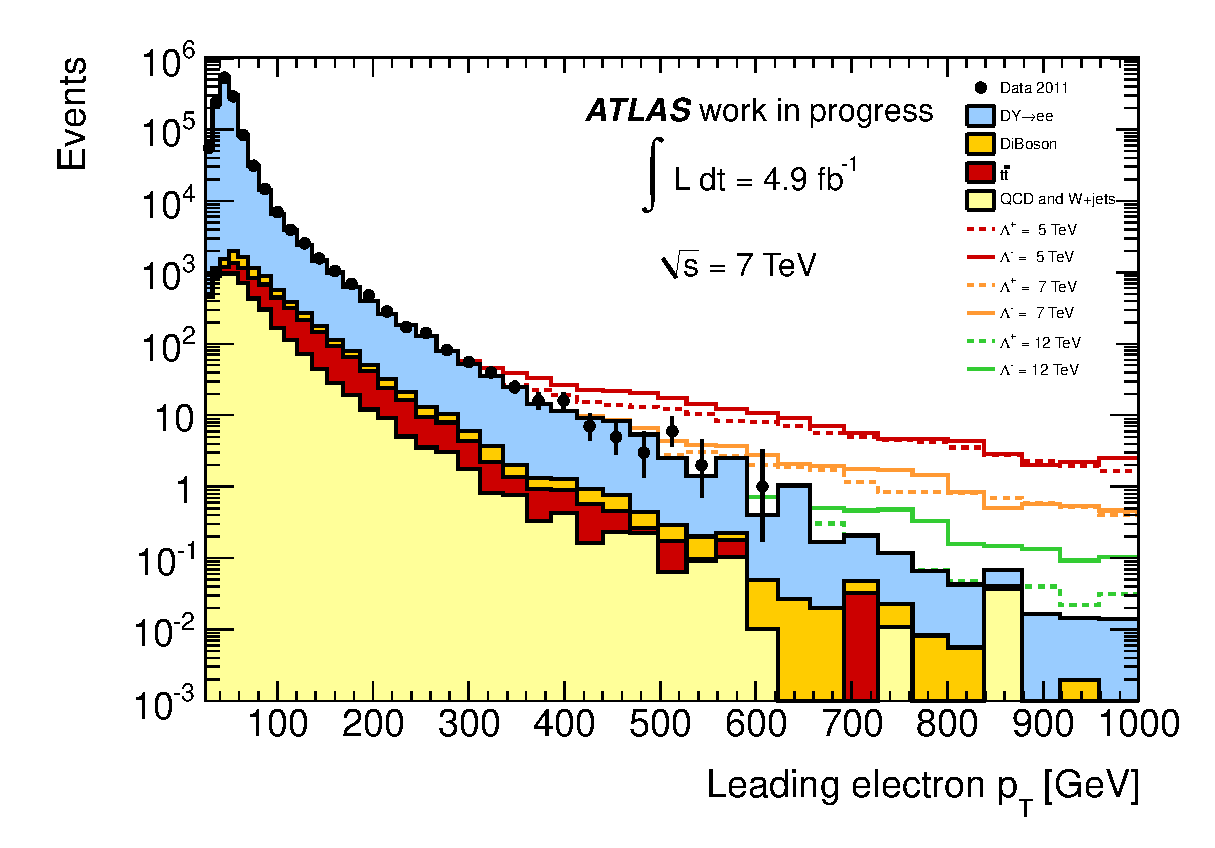
\includegraphics[width=0.49\linewidth]{images/lead_pT.eps}
	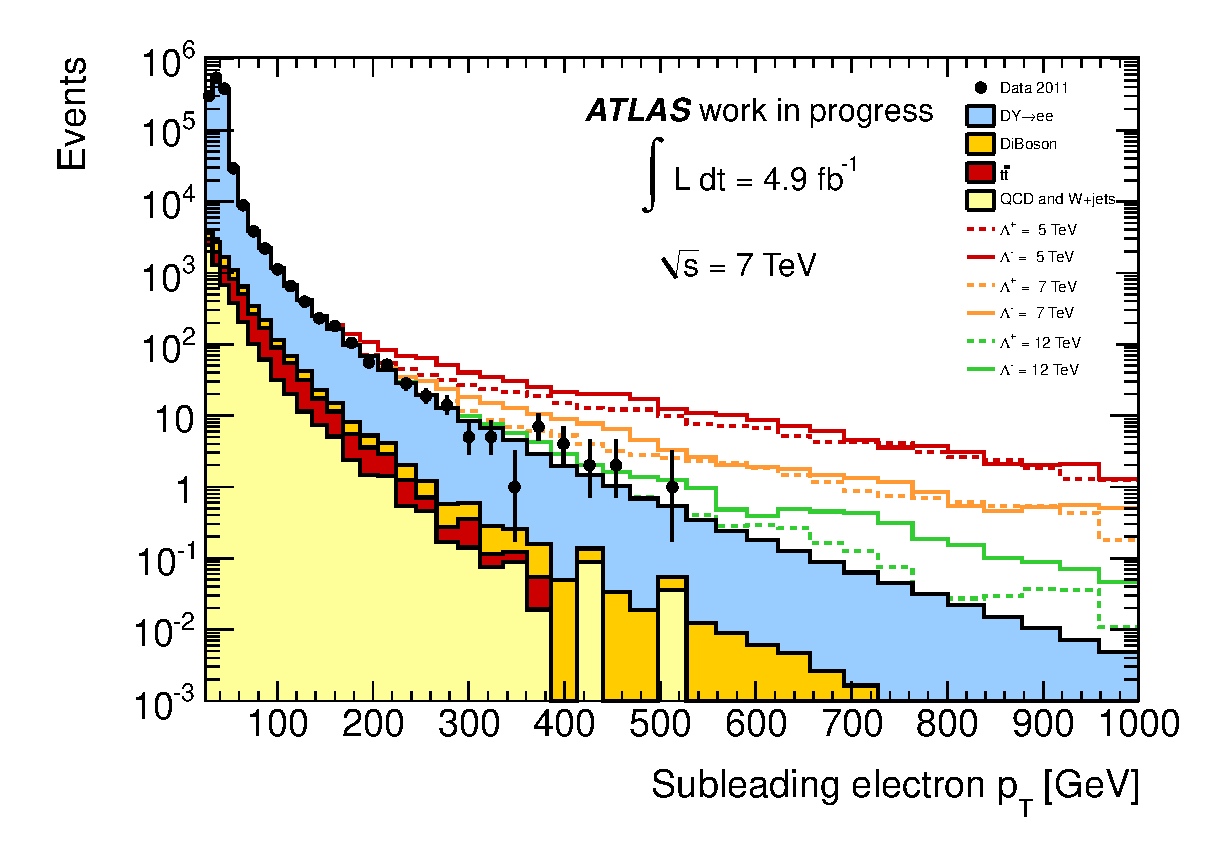
\includegraphics[width=0.49\linewidth]{images/sub_pT.eps}
	\caption{$p_{T}$ distribution of the leading (left) and subleading (right) electrons showing data, MC background and example CI signal samples compared to data.}
	\label{fig:CIpT}
	\end{figure}

	\begin{figure}[h!]
	\centering
	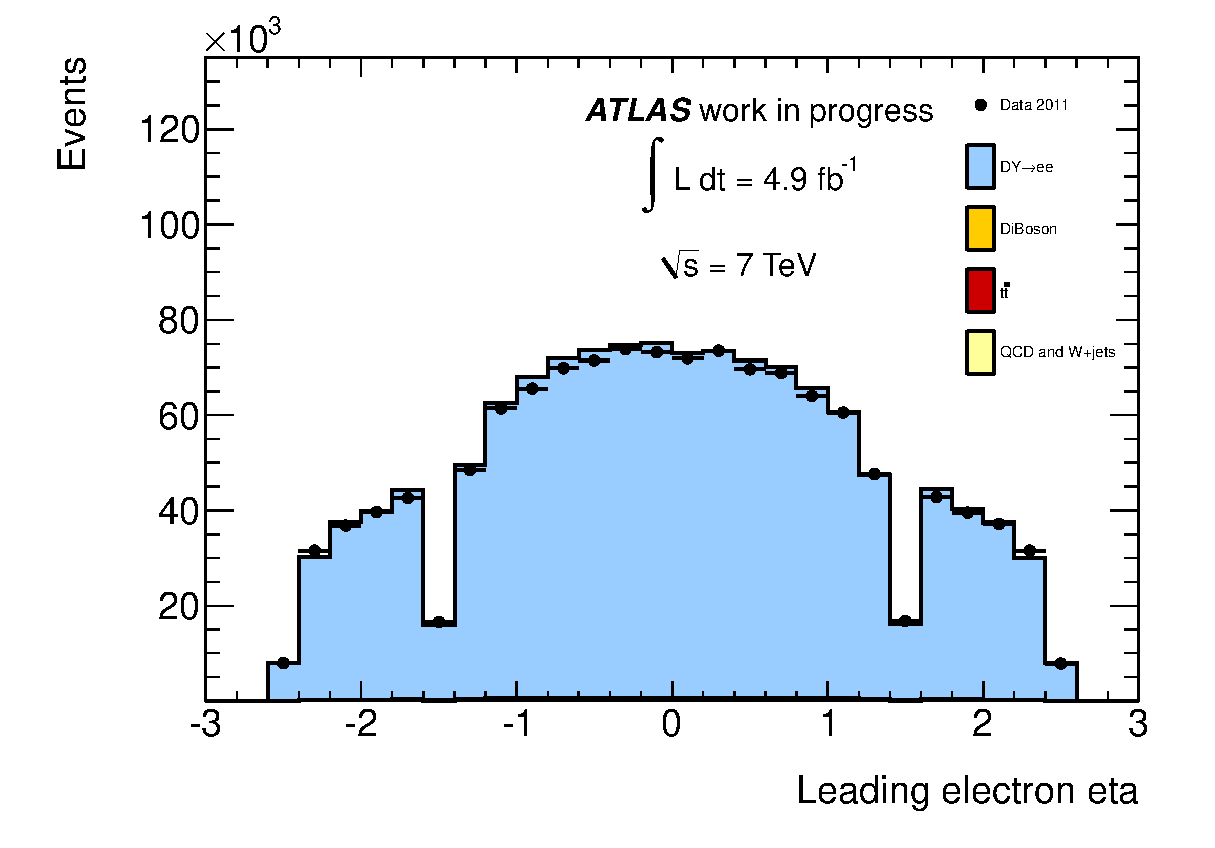
\includegraphics[width=0.49\linewidth]{images/lead_eta.eps}
	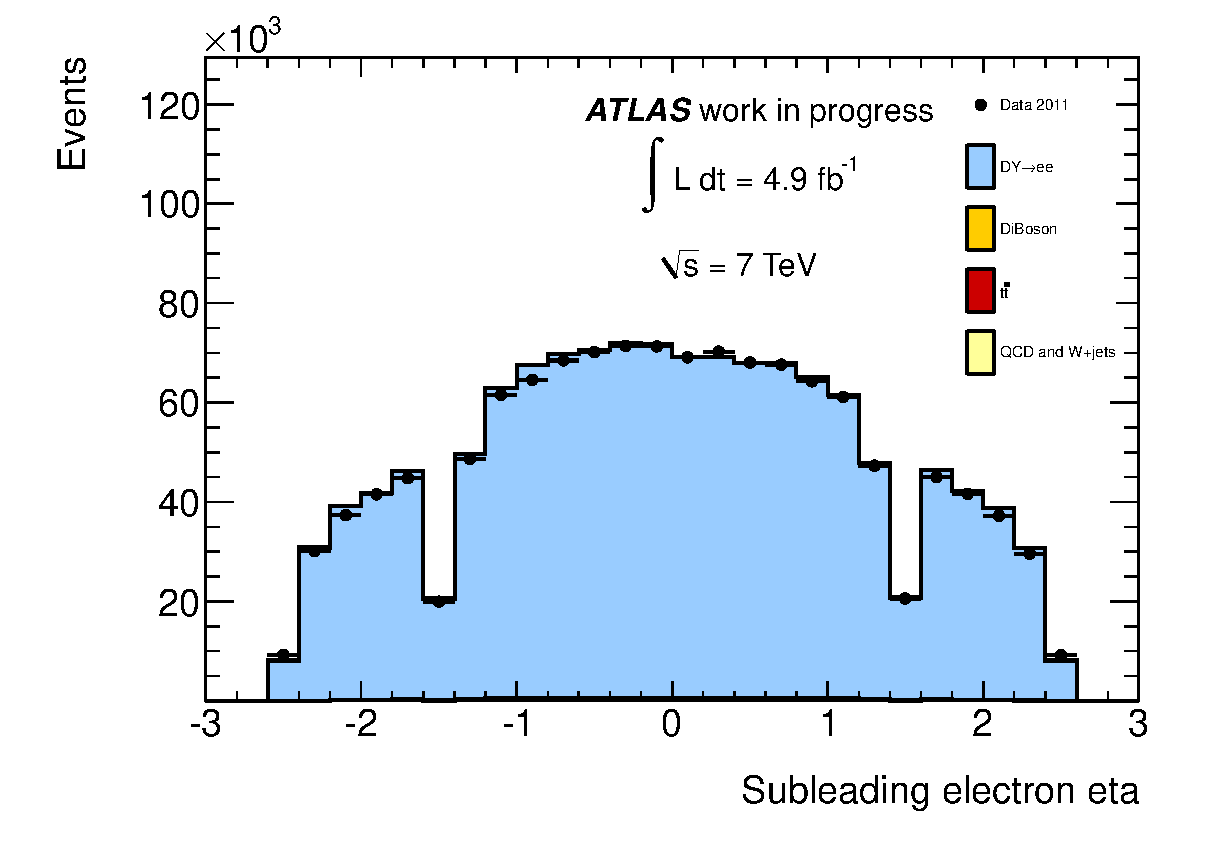
\includegraphics[width=0.49\linewidth]{images/sub_eta.eps}
	\caption{$\eta$ distribution of the leading (left) and subleading (right) electrons showing data, MC background compared to data.}
	\label{fig:eta}
	\end{figure}

	Control plots were produced to display that the distributions were behaving as predicted such as the $p_{T}$ (Fig. \ref{fig:CIpT}) and the $\eta$ (Fig. \ref{fig:eta}) distributions.





\subsection{New Physics Signal Expectation}
%(analysis method)

	\begin{table}[h!]
	\centering % centering table
	\begin{tabular}{l ccccc} % creating eight columns
	\hline\hline \\[-2ex] %inserting double-line
	$m_{ee}$ [GeV] & 110-200 & 200-400 & 400-800 & 800-1200 & 1200-3000 \\ [0.2ex]
	\hline  \\[-2ex] % inserts single-line
	$\Lambda^{-} = 3$ TeV & 18790.8 $\pm$ 137.1 & 5022.4 $\pm$ 70.9 & 2766.3 $\pm$ 52.6 & 1089.2 $\pm$ 33.0 & 673.3 $\pm$ 25.9 \\ 
	$\Lambda^{-} = 4$ TeV & 18212.5 $\pm$ 135.0 & 3707.1 $\pm$ 60.9 & 1102.5 $\pm$ 33.2 & 356.9 $\pm$ 18.9 & 214.3 $\pm$ 14.6 \\ 
	$\Lambda^{-} = 5$ TeV & 17821.5 $\pm$ 133.5 & 3310.5 $\pm$ 57.5 & 653.1 $\pm$ 25.6 & 160.6 $\pm$ 12.7 & 97.7 $\pm$ 9.9 \\ 
	$\Lambda^{-} = 7$ TeV & 17711.1 $\pm$ 133.1 & 3018.8 $\pm$ 54.9 & 385.0 $\pm$ 19.6 & 56.1 $\pm$ 7.5 & 26.5 $\pm$ 5.1 \\ 
	$\Lambda^{-} = 12$ TeV & 17693.4 $\pm$ 133.0 & 2992.7 $\pm$ 54.7 & 296.5 $\pm$ 17.2 & 20.4 $\pm$ 4.5 & 5.6 $\pm$ 2.4 \\ 
	\hline  \\[-2ex] % inserts single-line
	$\Lambda^{+} = 3$ TeV & 18106.6 $\pm$ 134.6 & 4063.8 $\pm$ 63.7 & 2103.3 $\pm$ 45.9 & 918.1 $\pm$ 30.3 & 621.4 $\pm$ 24.9 \\ 
	$\Lambda^{+} = 4$ TeV & 17958.1 $\pm$ 134.0 & 3178.6 $\pm$ 56.4 & 765.6 $\pm$ 27.7 & 288.0 $\pm$ 17.0 & 194.9 $\pm$ 14.0 \\ 
	$\Lambda^{+} = 5$ TeV & 18026.6 $\pm$ 134.3 & 2895.6 $\pm$ 53.8 & 432.1 $\pm$ 20.8 & 111.4 $\pm$ 10.6 & 78.8 $\pm$ 8.9 \\ 
	$\Lambda^{+} = 7$ TeV & 17926.4 $\pm$ 133.9 & 2857.5 $\pm$ 53.5 & 278.2 $\pm$ 16.7 & 34.3 $\pm$ 5.9 & 19.1 $\pm$ 4.4 \\ 
	\hline\hline  \\ %[0.2ex] %inserting double-line
	\end{tabular}
	\caption{Table of CI signal yields for 4.9 $fb^{-1}$.} %title of the table
	\label{tab:CIyeilds}
	\end{table}

	\begin{table}[h!]
	\centering % centering table
	\begin{tabular}{l c} % creating eight columns
	\hline\hline \\[-2ex] %inserting double-line
	$m_{ee}$ [GeV] & $\geq 1300$ \\  [0.2ex]
	\hline  \\[-2ex] % inserts single-line
	$M_{S} = 1500$ GeV (GRW) & 94.8 $\pm$ 9.7 \\ 
	$M_{S} = 2000$ GeV (GRW) & 42.7 $\pm$ 6.5 \\ 
	$M_{S} = 2500$ GeV (GRW) & 11.3 $\pm$ 3.4 \\ 
	$M_{S} = 3000$ GeV (GRW) & 3.2 $\pm$ 1.8 \\ 
	\hline\hline  \\ %[0.2ex] %inserting double-line
	\end{tabular}
	\caption{Table of ADD analysis region yields for 4.9 $fb^{-1}$.} %title of the table
	\label{tab:ADDyeilds}
	\end{table}


	Tables \ref{tab:CIyeilds} and \ref{tab:ADDyeilds} show the yeild from the CI and ADD MC signals used after scaling to data luminosity. The ADD yield is only shown in a single bin above 1300 GeV as the ADD statistical analysis uses only a one bin approach to set a limit of a general increase over SM background. Table \ref{tab:dataMCADDyeilds} shows the same one bin approach to the data MC comparison table.

	\begin{table}[h!]
	\centering % centering table
	\begin{tabular}{l c} % creating eight columns
	\hline\hline \\[-2ex] %inserting double-line
	$m_{ee}$ [GeV] & $\geq 1300$ \\  [0.2ex]
	\hline  \\[-2ex] % inserts single-line
	DY & 1.1 $\pm$ 1.1 \\ 
	$t\bar{t}$ & 0.0 $\pm$ 0.1 \\ 
	Dibosons & 0.1 $\pm$ 0.3 \\ 
	QCD + W+jets & 0.2 $\pm$ 0.4 \\ 
	\hline  \\[-2ex] % inserts single-line
	Total & 1.4 $\pm$ 1.2 \\ 
	\hline  \\[-2ex] % inserts single-line
	Data & 2.0 \\ 
	\hline\hline  \\ %[0.2ex] %inserting double-line
	\end{tabular}
	\caption{Table of data and MC yields for ADD analysis region.} %title of the table
	\label{tab:dataMCADDyeilds}
	\end{table}


	%\begin{table}[h!]
	%\centering % centering table
	%\begin{tabular}{l ccc}
	%\hline\hline \\[-2ex]
	%$\Lambda^{-} =$ & truth A & offline $\epsilon$ & $A~\times~\epsilon$ \\
	%\hline \\[-2ex]
	%3 TeV\\
	%4 TeV\\
	%5 TeV\\
	%7 TeV\\
	%12 TeV\\
	%\hline \\[-2ex]
	%$\Lambda^{+} =$ \\
	%\hline \\[-2ex]
	%3 TeV\\
	%4 TeV\\
	%5 TeV\\
	%7 TeV\\
	%12 TeV\\
	%\hline\hline \\
	%\end{tabular}
	%\caption{Table showing Acceptance*Efficency of CI signal samples} %title of the table
	%\label{tab:CIAxe}
	%\end{table}

	%\begin{table}[h!]
	%\centering % centering table
	%\begin{tabular}{l ccc}
	%\hline\hline \\[-2ex]
	%$M_{S} =$ & truth A & offline $\epsilon$ & $A~\times~\epsilon$ \\
	%\hline \\[-2ex]
	%1500 GeV \\
	%2000 GeV \\
	%2500 GeV \\
	%3000 GeV \\
	%\hline\hline \\
	%\end{tabular}
	%\caption{Table showing Acceptance*Efficency of CI signal samples} %title of the table
	%\label{tab:ADDAxe}
	%\end{table}

	%Acceptance and efficiency of selection of the signal samples was calculated (tables \ref{tab:CIAxe} and \ref{tab:ADDAxe}).


	\begin{figure}[h!p]
	\centering
	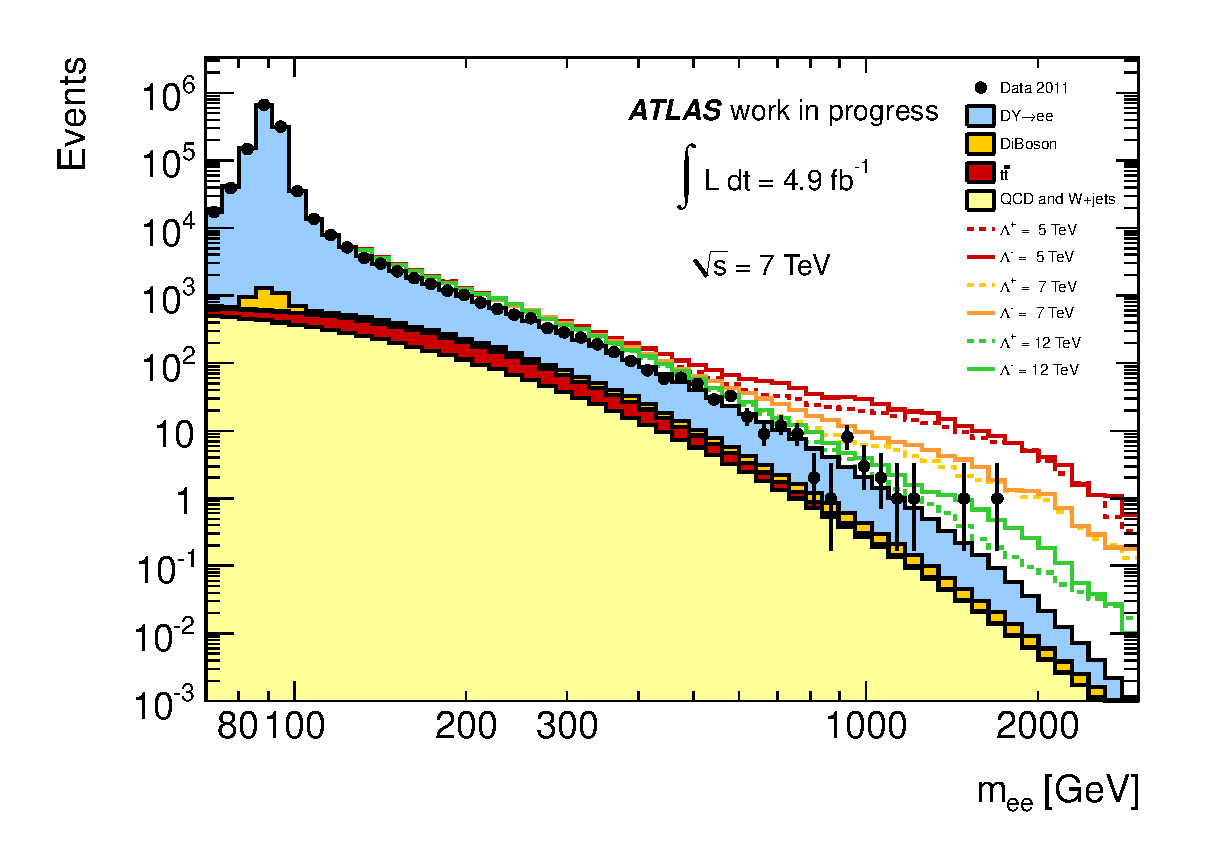
\includegraphics[width=0.7\linewidth]{images/inv_mass.eps}
	\caption{Dielectron invariant mass distribution for data and Monte Carlo simulation. Lines show expected distributions for the pressence of Contact Interactions.}
	\label{fig:CIinvMass}
	\end{figure}

	\begin{figure}[h!p]
	\centering
	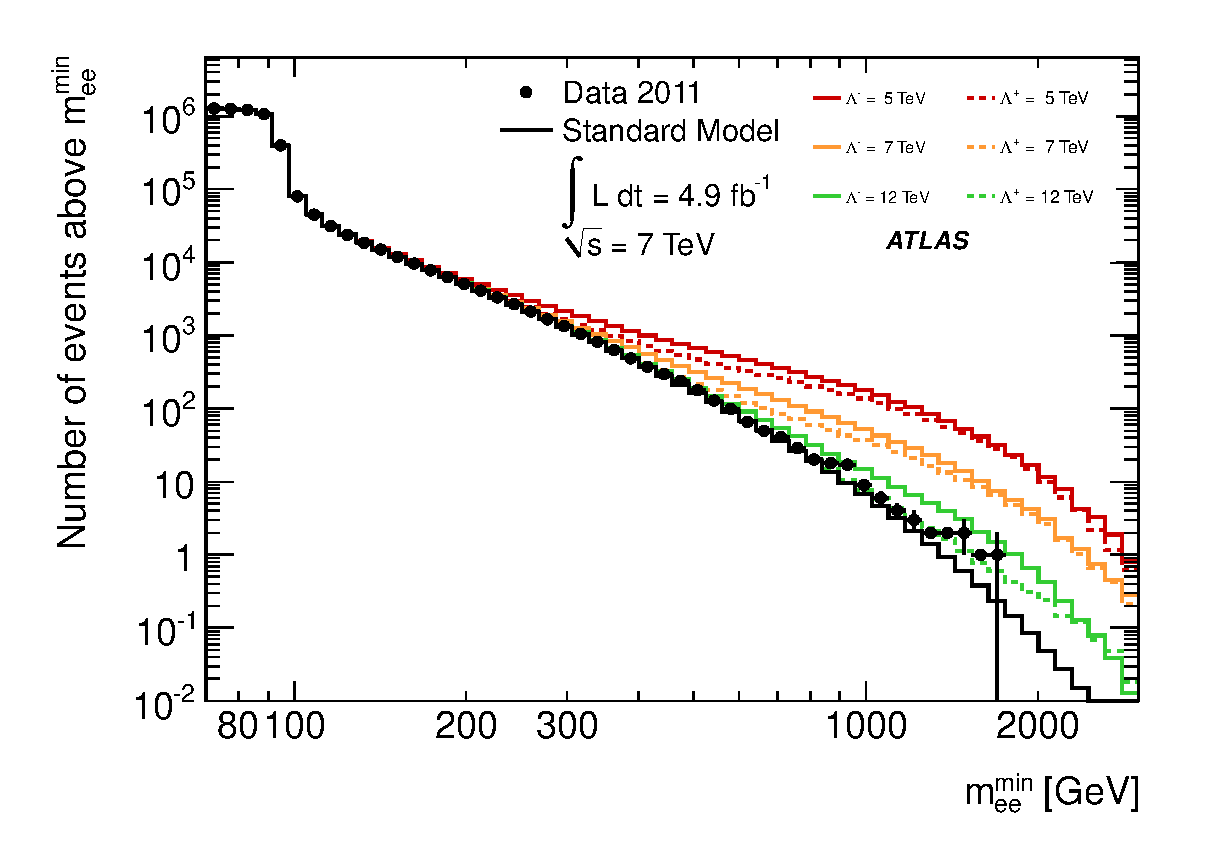
\includegraphics[width=0.7\linewidth]{images/int_inv_mass.eps}
	\caption{Dielectron intergrated invariant mass distribution for data and total background Monte Carlo simulation. Lines show expected distributions for the presence of Contact Interactions.}
	\label{fig:CIintinvMass}
	\end{figure}

	\begin{figure}[h!p]
	\centering
	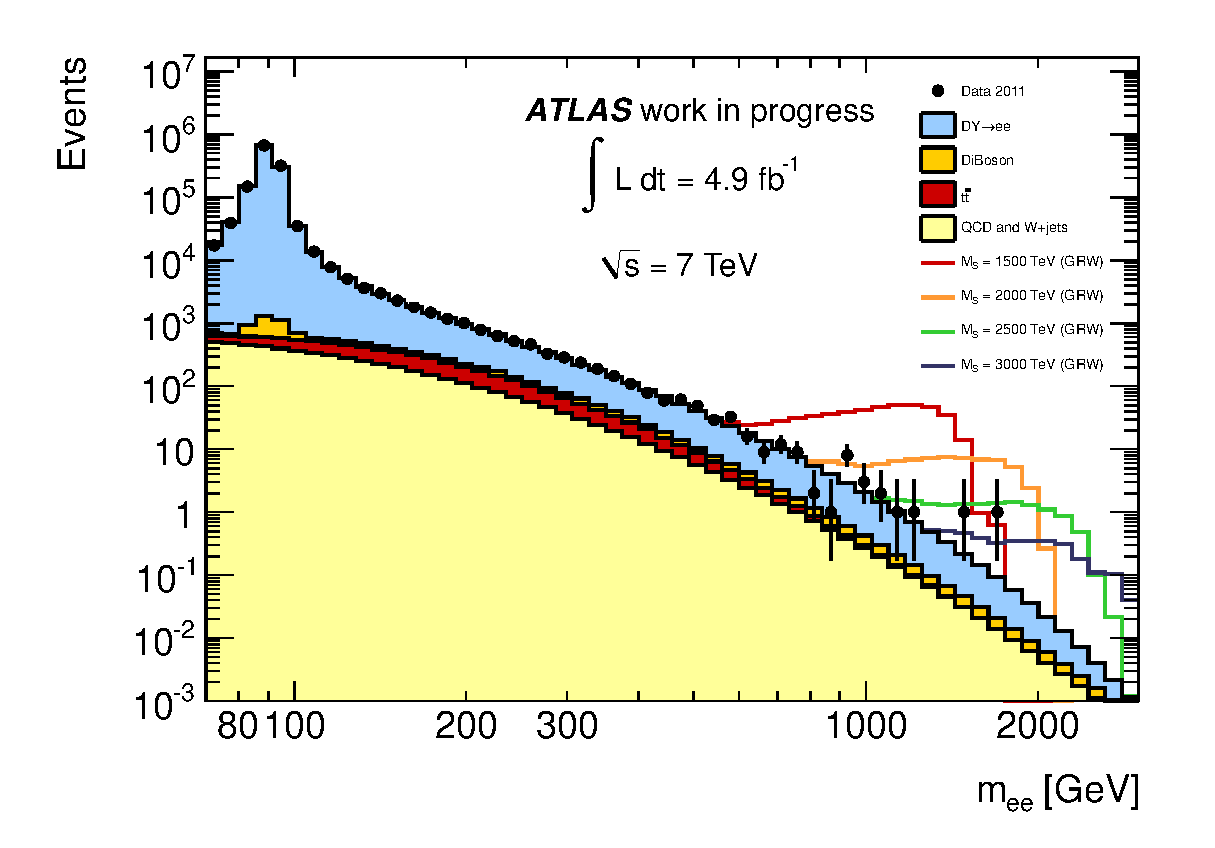
\includegraphics[width=0.7\linewidth]{images/ADD_inv_mass.eps}
	\caption{Dielectron invariant mass distribution for data and Monte Carlo simulation. Lines show expected distributions for the pressence of ADD.}
	\label{fig:ADDinvMass}
	\end{figure}

	\begin{figure}[h!p]
	\centering
	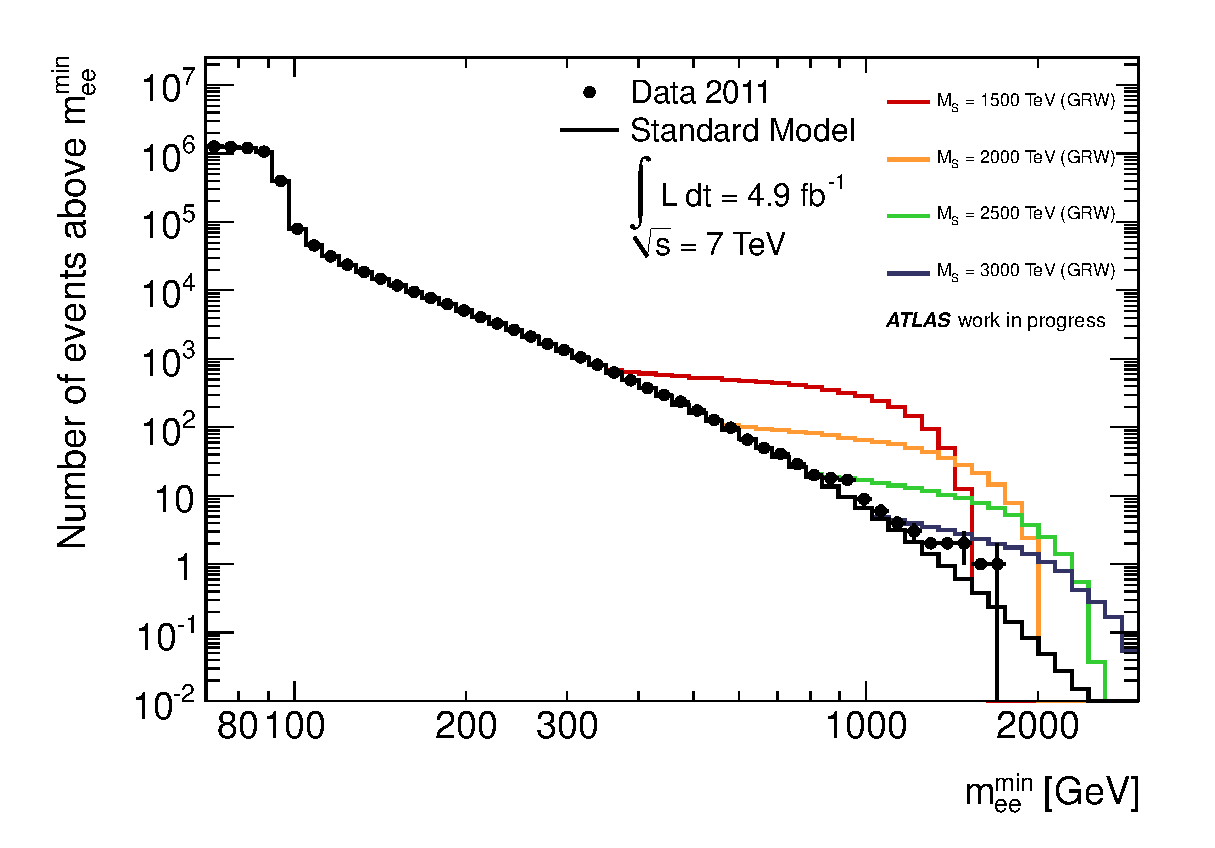
\includegraphics[width=0.7\linewidth]{images/ADD_int_inv_mass.eps}
	\caption{Dielectron intergrated invariant mass distribution for data and total backpacking Monte Carlo simulation. Lines show expected distributions for the presence of ADD.}
	\label{fig:ADDintinvMass}
	\end{figure}


	Figures \ref{fig:CIinvMass} (\ref{fig:ADDinvMass}) show the dielectron invariant mass distribution comparing data to background MC while showing the effect CI (ADD) would have on this spectrum. Figures \ref{fig:CIintinvMass} (\ref{fig:ADDintinvMass}) then show the same spectrum but with an intergrated invariant mass distribution instead which indicates better general increases in the dielectron spectrum.





\section{Statistical Analysis}

	If no evidence for new physics is found then a Bayesian counting method can be used to set a limit on the scale ($\Lambda$) of new physics. A comparison between the observed events yields and expected yield for a range of different CI benchmarks is done using 

	\begin{equation}
	        \mu = n_{DY+CI}(\theta,\bar{\nu}) + n_{non-DY bg}(\bar{\nu}),
	\end{equation}

	where $\mu$ is the number of expected events in each mass bin and n$_{DY+CI}$ and n$_{non-DY}$ are the number of events predicted by a particular benchmark signal sample and the number of predicted non DY background events respectively. $\nu$ is a set of Gaussian nuisance parameters that account for systematic uncertainties in the analysis while $\theta$ corresponds to the energy scale $\Lambda$.
	The likelihood function for observing a set of $\bar{n}$ events in $N$ mass bins is therefore given by: 

	\begin{equation}
	        \mathcal{L} (\bar{n}~|~\theta,\bar{\nu}) = \prod_{k=1}^{N} \frac{ \mu_{k}^{n_{k}} e^{-\mu_{k}} }{n_{k}!}
	\end{equation}

	as a product of Poission probabilities for each mass bin $k$. Using Bayes' theorem this gives posterior probability

	\begin{equation}
	        \mathcal{P}(\theta~|~\bar{n}) = \frac{1}{\mathcal{Z}} \mathcal{L}_{M}(\bar{n}~|~\theta)P(\theta)
	\end{equation}

	where Z is a normalisation constant and $\mathcal{L_{M}}$ is the marginalised likelihood after all nuisance parameters have been integrated out. A prior probability for $P(\theta)$ is chosen to be flat in $1/\Lambda^{2}$, motivated by the CI differential cross-section (Eq. \ref{eq:DiffCross}).

	A 95\% confidence level (CL) limit is found by finding $\Lambda_{lim}$ that satisfies $\int_{0} ^{\theta_{lim}} P(\theta~|~\bar{n}) d\theta = 0.95$ with $\theta = 1/\Lambda^{2}$. For this analysis the Bayesian Analysis Toolkit (BAT) \cite{BAT} was used to do this calculation. 









\section{Results}

	Results for the 2011 analysis are currently undergoing approval from ATLAS. Therefore the results presented here are provisional limits. 

	\begin{table}[h!]
	\centering % centering table
	\begin{tabular}{l ccc} % creating eight columns
	\hline\hline \\[-2ex] %inserting double-line
	Channel & ee & $\mu\mu$ & ee+$\mu\mu$\\  [0.2ex]
	\hline  \\[-2ex] % inserts single-line
	Expected CI constructive & 13.73 TeV & 12.24 TeV & 15.10 TeV\\ 
	Expected CI destructive & 10.41 TeV & 10.23 TeV & 11.42 TeV \\ 
	\hline  \\[-2ex] % inserts single-line
	Observed CI constructive & 11.60 TeV & 12.07 TeV & 12.70 TeV \\ 
	Observed CI destructive & 8.76 TeV & 9.17 TeV & 9.63 TeV \\ 
	\hline\hline  \\[-2ex] % inserts single-line
	Expected ADD & 2.84 TeV & 2.71 TeV & 2.94 TeV \\ 
	\hline  \\[-2ex] % inserts single-line
	Observed ADD & 2.71 TeV & 2.72 TeV & 2.94 TeV \\ 
	\hline\hline  \\ %[0.2ex] %inserting double-line
	\end{tabular}
	\caption{Table of 95\% confidence level limits found in the CI and ADD analyses} %title of the table
	\label{tab:CILimits}
	\end{table}

	An expected limit was obtained for the data set by generating 1000 Standard Model like pseudoexperiments. The Baysian limit setting method is then applied to each of these 1000 pseudoexperiments to get a distribution of $95\%$ CL limits. The median of these distributions is then taken as the expected limit for each channel. These results can be seen in table \ref{tab:CILimits} in which the expected limits are generally found to be higher because they dictate a scenario where no deviation from the Standard model background is found. In reality slight statistical fluctuations are found in the data set and so limits seen are lower than expected. 

	These limits are found to be higher than the limits in the last iteration of this analysis seen in the paper provided and the first limits set by ATLAS on ADD.



